\documentclass{report}

\usepackage{amsmath, amssymb}
\usepackage{ctex}
\usepackage[total={7in, 9.6in}]{geometry}
\usepackage{enumitem}
\usepackage{multicol}
\usepackage{tikz}

\newcommand{\sol}{\vspace{0.2cm}\textbf{解}:}
\pagenumbering{gobble}

\begin{document}
\setcounter{chapter}{8}
\setcounter{section}{3}

\section{三角函数的积化和差}

\subsection*{(选择题)}

\allowdisplaybreaks
    \begin{enumerate}[leftmargin=*]
        \item $\sin 52 \dfrac{1}{2}^{\circ} \cdot \cos 7 \dfrac{1}{2}^{\circ}=$ ?
        
        \sol{}
        \begin{align*}
            \sin 52 \dfrac{1}{2}^{\circ} \cdot \cos 7 \dfrac{1}{2}^{\circ} &= \dfrac{1}{2} \left[\sin \left(52 \dfrac{1}{2}^{\circ}+7 \dfrac{1}{2}^{\circ}\right)+\sin \left(52 \dfrac{1}{2}^{\circ}-7 \dfrac{1}{2}^{\circ}\right)\right] \\
            &= \dfrac{1}{2} (\sin 60^{\circ}+\sin 45^{\circ}) \\
            &= \dfrac{1}{2} \left(\dfrac{\sqrt{3}}{2}+\dfrac{\sqrt{2}}{2}\right) \\
            &= \dfrac{\sqrt{3}+\sqrt{2}}{4} &\blacksquare
        \end{align*}
    \end{enumerate}

\subsection*{(作答题)}
\begin{enumerate}[leftmargin=*]
    \item 试证 $\sec \left(\dfrac{\pi}{4}+\theta\right) \sec \left(\dfrac{\pi}{4}-\theta\right)=2 \sec 2 \theta$。
    
    \sol{}
    \begin{align*}
        \sec \left(\dfrac{\pi}{4}+\theta\right) \sec \left(\dfrac{\pi}{4}-\theta\right) &= \dfrac{1}{\cos \left(\dfrac{\pi}{4}+\theta\right)\cos \left(\dfrac{\pi}{4}-\theta\right)} \\
        &= \dfrac{1}{\dfrac{\cos\left(\dfrac{\pi}{4}+\theta + \dfrac{\pi}{4}-\theta\right)+\cos\left(\dfrac{\pi}{4}+\theta - \dfrac{\pi}{4}+\theta\right)}{2}} \\
        &= \dfrac{2}{\cos \dfrac{\pi}{2}+\cos 2 \theta} \\
        &= \dfrac{2}{0+\cos 2 \theta} \\
        &= 2 \sec 2 \theta &\blacksquare
    \end{align*}

    \item 试证 $8 \cos \theta \cos 2 \theta \cos 3 \theta-\dfrac{\sin 7 \theta}{\sin \theta}=1$。
    \sol{}
    \begin{align*}
        8 \cos \theta \cos 2 \theta \cos 3 \theta-\dfrac{\sin 7 \theta}{\sin \theta} &= \dfrac{8\sin\theta\cos\theta\cos2\theta\cos3\theta-\sin7\theta}{\sin\theta} \\
        &= \dfrac{4\sin2\theta\cos2\theta\cos3\theta-\sin7\theta}{\sin\theta} \\
        &= \dfrac{2\sin4\theta\cos3\theta-\sin7\theta}{\sin\theta} \\
        &= \dfrac{\sin7\theta + \sin\theta - \sin7\theta}{\sin\theta} \\
        &= \dfrac{\sin\theta}{\sin\theta} \\
        &= 1 &\blacksquare
        \end{align*}
        \newpage
    \item \begin{enumerate}
        \item 证明 $\cot \left(\theta+15^{\circ}\right)-\tan \left(\theta-15^{\circ}\right)=\dfrac{4 \cos 2 \theta}{1+2 \sin 2 \theta}$;
        
        \sol{}
        \begin{align*}
            \cot \left(\theta+15^{\circ}\right)-\tan \left(\theta-15^{\circ}\right) &= \dfrac{\cos(\theta+15^{\circ})}{\sin(\theta+15^{\circ})}-\dfrac{\sin(\theta-15^{\circ})}{\cos(\theta-15^{\circ})} \\
            & = \dfrac{\cos(\theta+15^{\circ})\cos(\theta-15^{\circ})-\sin(\theta+15^{\circ})\sin(\theta-15^{\circ})}{\sin(\theta+15^{\circ})\cos(\theta-15^{\circ})} \\
            & = \dfrac{\dfrac{1}{2}(\cos 2\theta + \cos 30^{\circ})+\dfrac{1}{2}(\cos 2\theta - \cos 30^{\circ})}{\dfrac{1}{2}(\sin 2\theta + \sin 30^{\circ})} \\
            & = \dfrac{\cos 2\theta +\cos 2\theta}{\sin 2\theta + \sin 30^{\circ}} \\
            & = \dfrac{2\cos 2\theta}{\dfrac{2\sin 2\theta + 1}{2}} \\
            & = \dfrac{4\cos 2\theta}{1+2\sin 2\theta} &\blacksquare
        \end{align*}

        \item 据此, 设 $\theta=60^{\circ}$, 证明 $\tan 75^{\circ}=2+\sqrt{3}$。
        \sol{}
        \begin{align*}
            \cot(60^{\circ}+15^{\circ})-\tan(60^{\circ}-15^{\circ}) &= \dfrac{4\cos 120^{\circ}}{1+2\sin 120^{\circ}} \\
            \cot 75^{\circ}-\tan 45^{\circ} &= \dfrac{4\left(-\dfrac{1}{2}\right)}{1+2\left(\dfrac{\sqrt{3}}{2}\right)} \\
            \cot 75^{\circ}-1 &= \dfrac{-2}{1+\sqrt{3}} \\
            \cot 75^{\circ} &= \dfrac{-2 + 1 + \sqrt{3}}{1+\sqrt{3}} \\
            \cot 75^{\circ} &= \dfrac{\sqrt{3}-1}{\sqrt{3}+1} \\
            \tan 75^{\circ} &= \dfrac{\sqrt{3}+1}{\sqrt{3}-1} \\
            & = \dfrac{3 + 1 + 2\sqrt{3}}{3-1} \\
            & = 2+\sqrt{3} &\blacksquare
        \end{align*}
    \end{enumerate}
\end{enumerate}

\newpage
\section{三角函数的和差化积}

\subsection*{(选择题)}
\begin{enumerate}[leftmargin=*]
    \item $\cos ^2 \theta+\cos ^2\left(\theta+1^{\circ}\right)+\cos ^2\left(\theta+2^{\circ}\right)+\cdots+\cos ^2\left(\theta+179^{\circ}\right)$ 的值是
    
    \sol{}
    \begin{align*}
        \cos^2(\theta + 90^{ \circ}) &= (-\sin \theta)^2 = \sin^2 \theta \\
        \cos^2(\theta + 91^{ \circ}) &= (-\sin(\theta + 1^{ \circ}))^2 = \sin^2(\theta + 1^{ \circ}) \\
        &\ \ \vdots \\
        \cos^2(\theta + 179^{ \circ}) &= (-\sin(\theta + 89^{ \circ}))^2 = \sin^2(\theta + 89^{ \circ}) \\
        \\
        \cos^2 \theta+\cos^2(\theta+90^{ \circ}) &= \cos^2 \theta + \sin^2 \theta = 1 \\
        \cos^2(\theta+1^{ \circ})+\cos^2(\theta+91^{ \circ}) &= \cos^2(\theta+1^{ \circ}) + \sin^2(\theta+1^{ \circ}) = 1 \\
        &\ \ \vdots \\
        \cos^2(\theta+89^{ \circ})+\cos^2(\theta+179^{ \circ}) &= \cos^2(\theta+89^{ \circ}) + \sin^2(\theta+89^{ \circ}) = 1 
    \end{align*}
    $\therefore$ 原式 $= 1 \times 90 = 90$ \hfill $\blacksquare$

    \item $\cos ^2 2 x+2 \sin ^2 x$ 的极小值是
    
    \sol{}
    \begin{align*}
        \dfrac{d}{dx}(\cos^2 2x+2\sin^2 x) &= -4\sin 2x \cos 2x + 4\sin x \cos x \\
        &= -2\sin 4x + 2\sin 2x \\
        & = -2(\sin 4x - \sin 2x) \\
        & = -4\cos 3x \sin x \\
        \cos 3x \sin x &= 0 \\
        \cos 3x &= 0 \quad \text{ or } \quad \sin x = 0 \\
        3x &= \dfrac{\pi}{2} + k\pi \quad \text{ or } \quad x = k\pi \\
        x &= \dfrac{\pi}{6} + \dfrac{k\pi}{3} \quad \text{ or } \quad x = k\pi
    \end{align*}
    When $k = 0$, $x = \dfrac{\pi}{6}$ or $x = 0$; When $k = 1$, $x = \dfrac{\pi}{2}$ or $x = \pi$ \\
    \begin{align*}
        \dfrac{d^2}{dx^2}(\cos^2 2x+2\sin^2 x) &= -8\cos 4x + 4\cos 2x
    \end{align*}
    When $x = \dfrac{\pi}{6}$, $\dfrac{d^2}{dx^2} = 6$; When $x = 0$, $\dfrac{d^2}{dx^2} = -4$; When $x = \dfrac{\pi}{2}$, $\dfrac{d^2}{dx^2} = -12$; When $x = \dfrac{\pi}{6}$, $\dfrac{d^2}{dx^2} = 6$

    Hence, the minimum value is $\dfrac{3}{4}$ when $x = \dfrac{\pi}{6}$. \hfill $\blacksquare$

    \newpage
    \item 化简 $\cos \theta+\cos \left(\theta+\dfrac{2 \pi}{3}\right)+\cos \left(\theta+\dfrac{4 \pi}{3}\right)$。
    
    \sol{}
    \begin{align*}
        \cos \theta+\cos \left(\theta+\dfrac{2 \pi}{3}\right)+\cos \left(\theta+\dfrac{4 \pi}{3}\right) &= \cos \theta + 2\cos \left(\dfrac{\theta+\dfrac{2\pi}{3} + \theta + \dfrac{4\pi}{3}}{2}\right)\cos \left(-\dfrac{\pi}{3}\right) \\
        &= \cos \theta + \cos \left(\theta+\pi\right) \\
        &= \cos \theta - \cos \theta \\
        &= 0 &\blacksquare
    \end{align*}

    \item 已知 $\sin \alpha-\sin \beta=-\dfrac{1}{2}, \cos \alpha-\cos \beta=\dfrac{1}{2}$, 且 $\alpha$ 与 $\beta$ 都是锐角, 求 $\tan (\alpha-\beta)$ 的值。
    
    \sol{}
    \begin{align*}
        \sin \alpha-\sin \beta &= -\dfrac{1}{2}\\
        \sin^2 \alpha + \sin^2 \beta - 2\sin \alpha \sin \beta &= \dfrac{1}{4} \\
        \cos \alpha-\cos \beta &= \dfrac{1}{2} \\
        \cos^2 \alpha + \cos^2 \beta - 2\cos \alpha \cos \beta &= \dfrac{1}{4} \\
        2 - 2\sin \alpha \sin \beta - 2\cos \alpha \cos \beta &= \dfrac{1}{2} \\
        2 - 2\cos (\alpha - \beta) &= \dfrac{1}{2} \\
        \cos (\alpha - \beta) &= \dfrac{3}{4}
    \end{align*}
    $\because \sin\alpha - \sin\beta < 0$, $\therefore \alpha < \beta \implies \alpha - \beta < 0 \implies \alpha - \beta$ is in the fourth quadrant. \\
    \begin{center}
        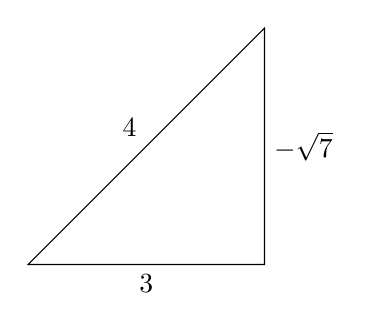
\begin{tikzpicture}
            \draw (0,0) -- (3,0) -- (3,3) -- cycle;
            \node at (1.5,0) [below] {$3$};
            \node at (3,1.5) [right] {$-\sqrt{7}$};
            \node at (1.5,1.5) [above left] {$4$};
        \end{tikzpicture}
    \end{center}
    \begin{align*}
        \tan (\alpha - \beta) &= -\dfrac{\sqrt{7}}{3} &\blacksquare
    \end{align*}

    \newpage
    \item 已知 $\sin \alpha+\sin \beta=\dfrac{1}{4}, \cos \alpha+\cos \beta=\dfrac{1}{3}$, 求 $\tan (\alpha+\beta)$ 的值。
    
    \sol{}
    \begin{align*}
        \sin \alpha+\sin \beta &= \dfrac{1}{4} \\
        2\sin\left(\dfrac{\alpha+\beta}{2}\right)\cos\left(\dfrac{\alpha-\beta}{2}\right) &= \dfrac{1}{4} \\
        \cos \alpha+\cos \beta &= \dfrac{1}{3} \\
        2\cos\left(\dfrac{\alpha+\beta}{2}\right)\cos\left(\dfrac{\alpha-\beta}{2}\right) &= \dfrac{1}{3} \\
        \dfrac{\sin\left(\dfrac{\alpha+\beta}{2}\right)}{\cos\left(\dfrac{\alpha+\beta}{2}\right)} &= \dfrac{3}{4} \\
        \tan\left(\dfrac{\alpha+\beta}{2}\right) &= \dfrac{3}{4}
        \end{align*}
        \begin{center}
            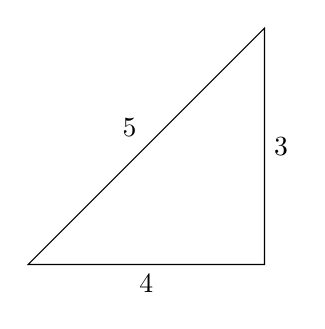
\begin{tikzpicture}
                \draw (0,0) -- (3,0) -- (3,3) -- cycle;
                \node at (1.5,0) [below] {$4$};
                \node at (3,1.5) [right] {$3$};
                \node at (1.5,1.5) [above left] {$5$};
            \end{tikzpicture}
        \end{center}
        \begin{align*}
            \sin(\alpha+\beta) &= 2\sin\left(\dfrac{\alpha+\beta}{2}\right)\cos\left(\dfrac{\alpha+\beta}{2}\right) \\
            & = 2 \times \dfrac{3}{5} \times \dfrac{4}{5} \\
            & = \dfrac{24}{25}
        \end{align*}
        \begin{center}
            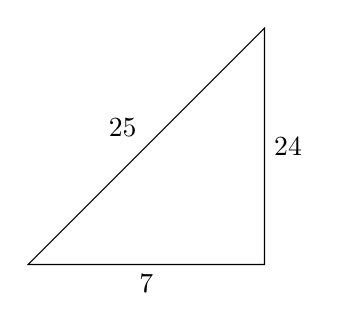
\begin{tikzpicture}
                \draw (0,0) -- (3,0) -- (3,3) -- cycle;
                \node at (1.5,0) [below] {$7$};
                \node at (3,1.5) [right] {$24$};
                \node at (1.5,1.5) [above left] {$25$};
            \end{tikzpicture}
        \end{center}
        \begin{align*}
            \tan(\alpha+\beta) &= \dfrac{24}{7} &\blacksquare
        \end{align*}

        \newpage
    \item 若 $\alpha+\beta=\dfrac{\pi}{3}$ 且 $y=\cos ^2 \alpha+\cos ^2 \beta$, 则 $y$ 的极大值是
    
    \sol{}
    \begin{align*}
        y &= \cos^2 \alpha + \cos^2 \beta \\
        &= \left(\cos \alpha + \cos \beta\right)^2 - 2\cos \alpha \cos \beta \\
        & = \left(2\cos \dfrac{\alpha + \beta}{2}\cos \dfrac{\alpha - \beta}{2}\right)^2 - \cos(\alpha + \beta) - \cos(\alpha - \beta) \\
        & = \left(2\cos \dfrac{\pi}{6}\cos \dfrac{\alpha - \beta}{2}\right)^2 - \cos\dfrac{\pi}{3} - \cos(\alpha - \beta) \\
        & = \left(\sqrt{3}\cos \dfrac{\alpha - \beta}{2}\right)^2 - \dfrac{1}{2} - \cos(\alpha - \beta) \\
        & = 3\cos^2 \dfrac{\alpha - \beta}{2} - \dfrac{1}{2} - \cos(\alpha - \beta) \\
        & = 3\left(\dfrac{1 + \cos(\alpha - \beta)}{2}\right) - \dfrac{1}{2} - \cos(\alpha - \beta) \\
        & = \dfrac{3}{2} + \dfrac{3}{2}\cos(\alpha - \beta) - \dfrac{1}{2} - \cos(\alpha - \beta) \\
        & = 1 + \dfrac{1}{2}\cos(\alpha - \beta) \\
    \end{align*}
    Since $-1 \leq \cos(\alpha - \beta) \leq 1$, the maximum value of $y$ is $\dfrac{3}{2}$ when $\cos(\alpha - \beta) = 1$. \hfill $\blacksquare$

    \item 已知 $\cos 2 \theta=5 \sin \theta-2$, 求 $\cos 2 \theta+\sin \theta$ 的值。
    
    \sol{}
    \begin{align*}
        \cos 2 \theta &= 5 \sin \theta - 2 \\
        1 - 2\sin^2 \theta &= 5\sin \theta - 2 \\
        2\sin^2 \theta + 5\sin \theta - 3 &= 0 \\
        (2\sin \theta - 1)(\sin \theta + 3) &= 0 \\
        \sin \theta &= \dfrac{1}{2} \quad \text{ or } \quad \sin \theta = -3 \text{ (rejected)} \\
        \cos 2 \theta + \sin \theta &= 5\sin \theta - 2 + \sin \theta \\
        & = 6\sin \theta - 2 = 1 &\blacksquare
    \end{align*}
    \item 化简 $\dfrac{\sin 13 x+\sin 7 x}{\cos 13 x+\cos 7 x}$。
    
    \sol{}
    \begin{align*}
        \dfrac{\sin 13 x+\sin 7 x}{\cos 13 x+\cos 7 x} &= \dfrac{2\sin 10 x \cos 3 x}{2\cos 10 x \cos 3 x} \\
        & = \dfrac{\sin 10 x}{\cos 10 x} \\
        & = \tan 10 x &\blacksquare
    \end{align*}
\end{enumerate}

\subsection*{(作答题)}
\begin{enumerate}[leftmargin=*]
    \item 设 $A+B+C=180^{\circ}$, 证明 $\sin A+\sin B+\sin C=4 \cos \dfrac{A}{2} \cos \dfrac{B}{2} \cos \dfrac{C}{2}$。
    
    \sol{}
    \begin{align*}
        A + B + C &= 180^{\circ} \\
        A + B &= 180^{\circ} - C \\
        \dfrac{A+B}{2} &= 90^{\circ} - \dfrac{C}{2} \\
        \sin \dfrac{A+B}{2} &= \cos \dfrac{C}{2} \\
        \sin A + \sin B + \sin C &= 2\sin \dfrac{A+B}{2}\cos \dfrac{A-B}{2} + 2\sin \dfrac{C}{2}\cos \dfrac{C}{2} \\
        & = 2\cos \dfrac{C}{2}\cos \dfrac{A-B}{2} + 2\sin \dfrac{C}{2}\cos \dfrac{C}{2} \\
        & = 2\cos \dfrac{C}{2}\left(\cos \dfrac{A-B}{2} + \sin \dfrac{C}{2}\right) \\
        & = 2\cos \dfrac{C}{2}\left(\cos \dfrac{A-B}{2} + \sin \left(90^{\circ} - \dfrac{A+B}{2}\right)\right) \\
        & = 2\cos \dfrac{C}{2}\left(\cos \dfrac{A-B}{2} + \cos \dfrac{A+B}{2}\right) \\
        & = 2\cos \dfrac{C}{2}\left(2\cos \dfrac{A}{2}\cos \dfrac{B}{2}\right) \\
        & = 4\cos \dfrac{A}{2}\cos \dfrac{B}{2}\cos \dfrac{C}{2} &\blacksquare
    \end{align*}

    \item 若 $A+B+C=180^{\circ}$, 利用两角和正切公式, 试证: $\tan A+\tan B+\tan C=\tan A \tan B \tan C$
    
    若 $\tan A=1, \tan B=2$, 求 $\angle C$。

    \sol{}
    \begin{align*}
        A + B + C &= 180^{\circ} \\
        A + B &= 180^{\circ} - C \\
        \tan(A + B) &= \tan(180^{\circ} - C) \\
        \tan(A + B) &= -\tan C \\
        \dfrac{\tan A + \tan B}{1 - \tan A \tan B} &= -\tan C \\
        \tan A + \tan B &= -\tan C + \tan A \tan B\tan C \\
        \tan A + \tan B + \tan C &= \tan A \tan B \tan C &\blacksquare\\
        \\
        \tan A + \tan B + \tan C &= \tan A \tan B \tan C \\
        1 + 2 + \tan C &= 2\tan C \\
        3 &= \tan C \\
        \angle C &= \arctan 3 = 71.57^{\circ} &\blacksquare
    \end{align*}

    \newpage
    \item 若 ${A}+{B}+{C}=180^{\circ}$, 试证 $\cos (B+C-A)+\cos (C+A-B)+\cos (A+B-C)=1+4 \cos A \cos B \cos C$。
    
    \sol{}
    \begin{align*}
       &\ \ \ \cos (B+C-A)+\cos (C+A-B)+\cos (A+B-C) \\
        &= \cos (180^{\circ}-A - A) + \cos (180^{\circ}-B - B) + \cos (180^{\circ}-C - C) \\
        & = -\cos 2A - \cos 2B - \cos 2C \\
        & = -(2\cos^2 A - 1) - 2\cos(B+C)\cos(B-C) \\
        & = -2\cos^2 A + 1 - 2\cos(180^{\circ}-A)\cos(B-C) \\
        & = -2\cos^2 A + 1 + 2\cos A\cos(B-C) \\
        & = 1 - 2\cos A[\cos A - \cos(B+C)] \\
        & = 1 - 2\cos A[\cos (180^{\circ}-(B+C)) - \cos(B+C)] \\
        & = 1 + 2\cos A[\cos(B+C) + \cos(B+C)] \\
        & = 1 + 4\cos A\cos B\cos C &\blacksquare
    \end{align*}
    \item 证明 $\sin \theta+\sin 2 \theta+\sin 4 \theta-\sin 7 \theta=4 \sin \dfrac{3 \theta}{2} \sin 3 \theta$。(Faulty Problem Statement)
    
    \sol{}
    \begin{align*}
        \sin \theta+\sin 2 \theta+\sin 4 \theta-\sin 7 \theta &= \sin \theta - 7\sin \theta + \sin 4\theta + \sin 2\theta \\
        & = -2\cos 4\theta\sin 3\theta + 2\sin 3\theta\cos\theta \\
        & = -2\sin 3\theta(\cos 4\theta - \cos \theta) \\
        & = 4\sin 3\theta\sin \dfrac{5\theta}{2}\sin \dfrac{3\theta}{2} &\blacksquare
    \end{align*}

    \item 如果 $A+B+C=180^{\circ}$, 试证 $\dfrac{1+\cos A-\cos B+\cos C}{1+\cos A+\cos B-\cos C}=\tan \dfrac{B}{2} \cot \dfrac{C}{2}$。
    
    \sol{}
    \begin{align*}
        A + B + C &= 180^{\circ} \\
        A + B &= 180^{\circ} - C \\
        \cos(A + B) &= \cos(180^{\circ} - C) \\
        \cos(A + B) &= -\cos C \\
        \dfrac{1 + \cos A - \cos B + \cos C}{1 + \cos A + \cos B - \cos C} &= \dfrac{2\sin^2 \dfrac{B}{2} + 2\cos\dfrac{A+C}{2}\cos\dfrac{A-C}{2}}{2\sin^2 \dfrac{C}{2} + 2\cos\dfrac{A+B}{2}\cos\dfrac{A-B}{2}} \\
        & = \dfrac{2\sin^2 \dfrac{B}{2} + 2\cos\left(90^{\circ} - \dfrac{B}{2}\right)\cos\left(\dfrac{A-C}{2}\right)}{2\sin^2 \dfrac{C}{2} + 2\cos\left(90^{\circ} - \dfrac{C}{2}\right)\cos\left(\dfrac{A-B}{2}\right)} \\
        & = \dfrac{2\sin^2 \dfrac{B}{2} + 2\sin\dfrac{B}{2}\cos\left(\dfrac{A-C}{2}\right)}{2\sin^2 \dfrac{C}{2} + 2\sin\dfrac{C}{2}\cos\left(\dfrac{A-B}{2}\right)} \\
        & = \dfrac{\sin\dfrac{B}{2}\left(\sin\dfrac{B}{2} + \cos\left(\dfrac{A-C}{2}\right)\right)}{\sin\dfrac{C}{2}\left(\sin\dfrac{C}{2} + \cos\left(\dfrac{A-B}{2}\right)\right)} \\
        & = \dfrac{\sin\dfrac{B}{2}\left(\sin\left(90^{\circ} - \dfrac{A+C}{2}\right) + \cos\left(\dfrac{A-C}{2}\right)\right)}{\sin\dfrac{C}{2}\left(\sin\left(90^{\circ} - \dfrac{A+B}{2}\right) + \cos\left(\dfrac{A-B}{2}\right)\right)} \\
        & = \dfrac{\sin\dfrac{B}{2}\left(\cos\left(\dfrac{A+C}{2}\right) + \cos\left(\dfrac{A-C}{2}\right)\right)}{\sin\dfrac{C}{2}\left(\cos\left(\dfrac{A+B}{2}\right) + \cos\left(\dfrac{A-B}{2}\right)\right)} \\
        & = \dfrac{\sin\dfrac{B}{2}\left(2\cos\dfrac{A}{2}\cos\dfrac{C}{2}\right)}{\sin\dfrac{C}{2}\left(2\cos\dfrac{A}{2}\cos\dfrac{B}{2}\right)} \\
        & = \dfrac{\sin\dfrac{B}{2}\cos\dfrac{C}{2}}{\sin\dfrac{C}{2}\cos\dfrac{B}{2}} \\
        & = \tan\dfrac{B}{2}\cot\dfrac{C}{2} &\blacksquare
    \end{align*}

    \item 已知 $\sin {A}-\sin {B}=\dfrac{1}{2}$ 及 $\cos {A}-\cos {B}=-\dfrac{1}{3}$, 试求 $\sin ({A}+{B})$。
    \sol{}

    \begin{align*}
        \sin A - \sin B &= \dfrac{1}{2} \\
        2\cos\left(\dfrac{A+B}{2}\right)\sin\left(\dfrac{A-B}{2}\right) &= \dfrac{1}{2} \\
        \cos A - \cos B &= -\dfrac{1}{3} \\
        -2\sin\left(\dfrac{A+B}{2}\right)\sin\left(\dfrac{A-B}{2}\right) &= -\dfrac{1}{3} \\
        \dfrac{\sin\left(\dfrac{A+B}{2}\right)}{\cos\left(\dfrac{A+B}{2}\right)} &= \dfrac{2}{3} \\
        \tan\left(\dfrac{A+B}{2}\right) &= \dfrac{2}{3} \\
    \end{align*}
    \begin{center}
        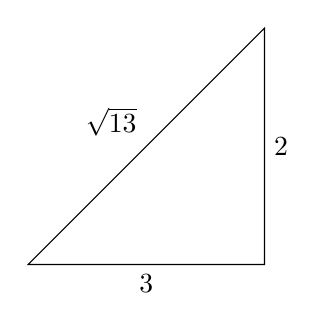
\begin{tikzpicture}
            \draw (0,0) -- (3,0) -- (3,3) -- cycle;
            \node at (1.5,0) [below] {$3$};
            \node at (3,1.5) [right] {$2$};
            \node at (1.5,1.5) [above left] {$\sqrt{13}$};
        \end{tikzpicture}
    \end{center}
    \begin{align*}
        \sin(A+B) &= 2\sin\left(\dfrac{A+B}{2}\right)\cos\left(\dfrac{A+B}{2}\right) \\
        & = 2 \times \dfrac{2}{\sqrt{13}} \times \dfrac{3}{\sqrt{13}} \\
        & = \dfrac{12}{13} &\blacksquare
    \end{align*}

    \item 证 $\dfrac{\sin \alpha+\sin 3 \alpha+\sin 5 \alpha+\sin 7 \alpha}{\cos \alpha+\cos 3 \alpha+\cos 5 \alpha+\cos 7 \alpha}=\tan 4 \alpha$。
    
    \sol{}
    \begin{align*}
        \dfrac{\sin \alpha+\sin 3 \alpha+\sin 5 \alpha+\sin 7 \alpha}{\cos \alpha+\cos 3 \alpha+\cos 5 \alpha+\cos 7 \alpha} &= \dfrac{2\sin 4\alpha\cos 3\alpha + 2\sin 4\alpha\cos \alpha}{2\cos 4\alpha\cos 3\alpha + 2\cos 4\alpha\cos \alpha} \\
        & = \dfrac{2\sin 4\alpha(\cos 3\alpha + \cos \alpha)}{2\cos 4\alpha(\cos 3\alpha + \cos \alpha)} \\
        & = \tan 4\alpha &\blacksquare
    \end{align*}

    \item 试证 $2 \sin ^2 3 \theta-2 \sin ^2 \theta=\cos 2 \theta-\cos 6 \theta$。
    
    以 $\theta=\dfrac{\pi}{10}$ 代入上式, 证明 $\sin \dfrac{3 \pi}{10}-\sin \dfrac{\pi}{10}=\dfrac{1}{2}$。
    
    [ 提示: 用 $\cos x=\sin \left(\dfrac{\pi}{2}-x\right)$ ]

    \sol{}
    \begin{align*}
        2 \sin ^2 \dfrac{3\pi}{10}-2 \sin ^2 \dfrac{\pi}{10} &= \cos \dfrac{\pi}{5}-\cos \dfrac{3\pi}{5} \\
        2\left(\sin^2 \dfrac{3\pi}{10} - \sin^2 \dfrac{\pi}{10}\right) &= 2\sin \dfrac{2\pi}{5}\sin \dfrac{\pi}{5} \\
        \sin^2 \dfrac{3\pi}{10} - \sin^2 \dfrac{\pi}{10} &= \sin \dfrac{2\pi}{5}\sin \dfrac{\pi}{5} \\
        \left(\sin \dfrac{3\pi}{10} - \sin \dfrac{\pi}{10}\right)\left(\sin \dfrac{3\pi}{10} + \sin \dfrac{\pi}{10}\right) &= \sin \dfrac{2\pi}{5}\sin \dfrac{\pi}{5} \\
        \left(\sin \dfrac{3\pi}{10} - \sin \dfrac{\pi}{10}\right)\left(2\sin\dfrac{\pi}{5}\cos\dfrac{\pi}{10}\right) &= \sin \dfrac{2\pi}{5}\sin \dfrac{\pi}{5} \\
        \left(\sin \dfrac{3\pi}{10} - \sin \dfrac{\pi}{10}\right)\left(2\sin\dfrac{\pi}{5}\sin\dfrac{2\pi}{5}\right) &= \sin \dfrac{2\pi}{5}\sin \dfrac{\pi}{5} \\
        2\left(\sin \dfrac{3\pi}{10} - \sin \dfrac{\pi}{10}\right) &= 1\\
        \sin \dfrac{3\pi}{10} - \sin \dfrac{\pi}{10} &= \dfrac{1}{2} &\blacksquare
    \end{align*}

    \item 在 $\triangle {ABC}$ 中, 试证明 $\dfrac{a+b}{c}=\dfrac{\sin {A}+\sin {B}}{\sin {C}}$。

    \sol{}
    \begin{align*}
        \dfrac{c}{\sin C} &= \dfrac{a}{\sin A} = \dfrac{b}{\sin B} = R\\
        a = R\sin A &\qquad b = R\sin B \qquad c = R\sin C \\
        \dfrac{a+b}{c} &= \dfrac{R\sin A + R\sin B}{R\sin C} = \dfrac{\sin A + \sin B}{\sin C} &\blacksquare
    \end{align*}
    
    \newpage
    若在这三角形中, $a+b=2 c$ 及 ${A}-{B}=90^{\circ}$,
    \begin{enumerate}
        \item 试证明 $\sin \dfrac{C}{2}=\dfrac{1}{2 \sqrt{2}}$;

        \sol{}
        \begin{align*}
            \dfrac{a+b}{c} & = \dfrac{\sin A + \sin B}{\sin C}\\
            \dfrac{2c}{c} & = \dfrac{\sin A + \sin B}{\sin C}\\
            2 & = \dfrac{\sin A + \sin B}{\sin C}\\
            2\sin C & = \sin A + \sin B\\
            2\sin C &= 2\sin\dfrac{A+B}{2}\cos\dfrac{A-B}{2} \\
            2\sin C &= 2\cos\dfrac{180^{\circ} - (A+B)}{2}\cos 45^{\circ} \\
            2\sin C &= \sqrt{2}\cos \dfrac{C}{2} \\
            4\sin\dfrac{C}{2}\cos{\dfrac{C}{2}} &= \sqrt{2}\cos \dfrac{C}{2} \\
            4\sin\dfrac{C}{2} &= \sqrt{2} \\
            \sin \dfrac{C}{2} &= \dfrac{\sqrt{2}}{4} = \dfrac{1}{2\sqrt{2}} &\blacksquare
        \end{align*}
        \item 求 ${A}, {B}$ 及 ${C}$ 的值。
        
        \sol{}
        \begin{align*}
            \sin \dfrac{C}{2} &= \dfrac{1}{2\sqrt{2}} \\
            \dfrac{C}{2} &= \arcsin \dfrac{1}{2\sqrt{2}} \\
            C &= 2\arcsin \dfrac{1}{2\sqrt{2}} &\blacksquare\\
            &= 41.41^{\circ} \\
            A + B + C &= 180^{\circ} \\
            A + B &= 180^{\circ} - 41.41^{\circ} \\
            & = 138.59^{\circ} \\
            A - B &= 90^{\circ} \\
            2A &= 228.59^{\circ} \\
            A &= 114.30^{\circ} &\blacksquare\\
            B &= 24.30^{\circ} &\blacksquare
        \end{align*}
    \end{enumerate}
    
    \newpage
    \item 若 $\sin 6 x=\dfrac{1}{\sin x}$, 证明 $\sin 5 x \sin 4 x-\sin 3 x \sin 2 x-\sin 8 x \sin x=1$。
    
    \sol{}
    \begin{align*}
        &\ \ \ \sin 5 x \sin 4 x-\sin 3 x \sin 2 x-\sin 8 x \sin x\\
        & = \dfrac{1}{2}\left[-\cos 9x + \cos x + \cos 5x - \cos x + \cos 9x - \cos 7x\right] \\
        & = -\dfrac{1}{2}(\cos 7x - \cos 5x) \\
        & = \sin 6x \sin x \\
        & = \dfrac{1}{\sin x} \cdot \sin x \\
        & = 1 &\blacksquare
    \end{align*}

    \item 在 $\triangle {ABC}$ 中, 试证 $4 \sin \dfrac{{A}}{2} \sin \dfrac{{B}}{2} \sin \dfrac{{C}}{2}=\cos {A}+\cos {B}+\cos {C}-1$。
    
    \sol{}
    \begin{align*}
        \cos {A}+\cos {B}+\cos {C} &= 2\cos \dfrac{A+B}{2}\cos \dfrac{A-B}{2} + 1 - 2\sin^2 \dfrac{C}{2} \\
        &= 2\cos \dfrac{180^{\circ}-C}{2}\cos \dfrac{A-B}{2} - 2\sin^2 \dfrac{C}{2} + 1 \\
        &= 2\sin \dfrac{C}{2}\cos \dfrac{A-B}{2} - 2\sin^2 \dfrac{C}{2} + 1 \\
        &= 2\sin \dfrac{C}{2}\left(\cos \dfrac{A-B}{2} - \sin \dfrac{C}{2}\right) + 1 \\
        &= 2\sin \dfrac{C}{2}\left(\cos \dfrac{A-B}{2} - \sin\dfrac{180^{\circ}-(A+B)}{2}\right) + 1 \\
        &= 2\sin \dfrac{C}{2}\left(\cos \dfrac{A-B}{2} - \cos \dfrac{A+B}{2}\right) + 1 \\
        &= 4\sin \dfrac{A}{2}\sin \dfrac{B}{2}\sin \dfrac{C}{2} + 1 \\
        4 \sin \dfrac{{A}}{2} \sin \dfrac{{B}}{2} \sin \dfrac{{C}}{2} &= \cos {A}+\cos {B}+\cos {C}-1 &\blacksquare
    \end{align*}
    \item 已知 $\sin \alpha+\sin \beta=\dfrac{1}{4}, \cos \alpha+\cos \beta=\dfrac{1}{3}$, 求 $\tan (\alpha+\beta)$ 的值。
    
    \sol{}
    \begin{align*}
        \sin \alpha+\sin \beta &= \dfrac{1}{4} \\
        2\sin\left(\dfrac{\alpha+\beta}{2}\right)\cos\left(\dfrac{\alpha-\beta}{2}\right) &= \dfrac{1}{4} \\
        \cos \alpha+\cos \beta &= \dfrac{1}{3} \\
        2\cos\left(\dfrac{\alpha+\beta}{2}\right)\cos\left(\dfrac{\alpha-\beta}{2}\right) &= \dfrac{1}{3} \\
        \tan\left(\dfrac{\alpha+\beta}{2}\right) &= \dfrac{3}{4}
        \end{align*}
        \begin{center}
            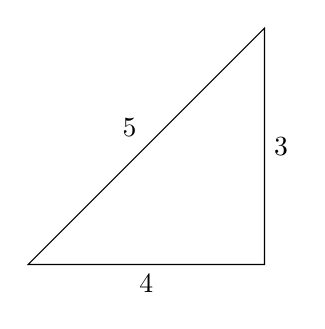
\begin{tikzpicture}
                \draw (0,0) -- (3,0) -- (3,3) -- cycle;
                \node at (1.5,0) [below] {$4$};
                \node at (3,1.5) [right] {$3$};
                \node at (1.5,1.5) [above left] {$5$};
            \end{tikzpicture}
        \end{center}
        \begin{align*}
            \sin(\alpha+\beta) &= 2\sin\left(\dfrac{\alpha+\beta}{2}\right)\cos\left(\dfrac{\alpha+\beta}{2}\right) \\
            & = 2 \times \dfrac{3}{5} \times \dfrac{4}{5} \\
            & = \dfrac{24}{25}
        \end{align*}
        \begin{center}
            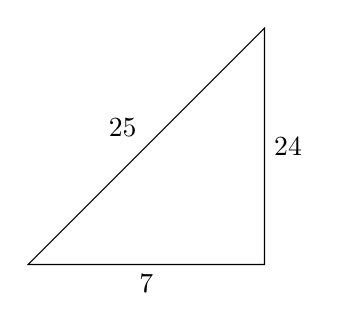
\begin{tikzpicture}
                \draw (0,0) -- (3,0) -- (3,3) -- cycle;
                \node at (1.5,0) [below] {$7$};
                \node at (3,1.5) [right] {$24$};
                \node at (1.5,1.5) [above left] {$25$};
            \end{tikzpicture}
        \end{center}
        \begin{align*}
            \tan(\alpha+\beta) &= \dfrac{24}{7} &\blacksquare
    \end{align*}

    \item 在 $\triangle {ABC}$ 中, 如果 $\sin {A}$、 $\sin {B}$ 及 $\sin {C}$ 成等差数列, 试证 $\cot \dfrac{{A}}{2} \cot \dfrac{{C}}{2}=3$。
    
    \sol{}
    \begin{align*}
        \sin B &= \dfrac{\sin A + \sin C}{2} \\
        \sin [180^{\circ} - (A + C)] &= \dfrac{\sin A + \sin C}{2} \\
        \sin (A + C) &= \dfrac{\sin A + \sin C}{2} \\
        \sin (A + C) &= \sin \dfrac{A + C}{2} \cos \dfrac{A - C}{2}\\
        2\sin \dfrac{A + C}{2} \cos \dfrac{A + C}{2} &= \sin \dfrac{A + C}{2} \cos \dfrac{A - C}{2} \\
        2\cos \dfrac{A + C}{2} &= \cos \dfrac{A - C}{2} \\
        \cot \dfrac{A}{2} \cot \dfrac{C}{2} &= \dfrac{\cos \dfrac{A}{2} \cos \dfrac{C}{2}}{\sin \dfrac{A}{2} \sin \dfrac{C}{2}} = \dfrac{\cos\dfrac{A+C}{2} + \cos\dfrac{A-C}{2}}{\cos\dfrac{A-C}{2} - \cos\dfrac{A+C}{2}} \\
        & = \dfrac{\cos\dfrac{A+C}{2} + 2\cos \dfrac{A + C}{2}}{2\cos \dfrac{A + C}{2} - \cos\dfrac{A+C}{2}} \\
        & = \dfrac{3\cos \dfrac{A + C}{2}}{\cos \dfrac{A + C}{2}} = 3 &\blacksquare
    \end{align*}

    \item 若 $A+B+C=180^{\circ}$ 且 $A \neq 90^{\circ}$, 证明 $\dfrac{\sin B}{\sin C}=\dfrac{\sin A \cos B-\sin C}{\sin A \cos C-\sin B}$
    
    \sol{}
    \begin{align*}
        \dfrac{\sin A \cos B-\sin C}{\sin A \cos C-\sin B} &= \dfrac{\sin A\cos B - \sin(180^{\circ} - (A + B))}{\sin A\cos C - \sin(180^{\circ} - (A + C))} \\
        & = \dfrac{\sin A\cos B - \sin(A + B)}{\sin A\cos C - \sin(A + C)} \\
        & = \dfrac{\sin A\cos B - \sin A\cos B - \cos A\sin B}{\sin A\cos C - \sin A\cos C - \cos A\sin C} \\
        & = \dfrac{-\cos A\sin B}{-\cos A\sin C} \\
        & = \dfrac{\sin B}{\sin C} &\blacksquare
    \end{align*}
\end{enumerate}

\end{document}
